%! Mode:: "TeX:UTF-8"
%! TEX program = xelatex
\PassOptionsToPackage{quiet}{xeCJK}
\documentclass[withoutpreface,bwprint]{cumcmthesis}
\usepackage{etoolbox}
\BeforeBeginEnvironment{tabular}{\zihao{-5}}
\usepackage[numbers,sort&compress]{natbib}  % 文献管理宏包
\usepackage[framemethod=TikZ]{mdframed}  % 框架宏包
\usepackage{url}  % 网页链接宏包
\usepackage{subcaption}  % 子图宏包
\newcolumntype{C}{>{\centering\arraybackslash}X}
\newcolumntype{R}{>{\raggedleft\arraybackslash}X}
\newcolumntype{L}{>{\raggedright\arraybackslash}X}

\title{全国大学生数学建模竞赛论文模板}  % 论文标题
\tihao{}  % 题号
\baominghao{}  % 报名号
\schoolname{}  % 学校
\membera{}  % 队员a
\memberb{}  % 队员b
\memberc{}  % 队员c
\supervisor{}  % 指导老师
\yearinput{}
\monthinput{}
\dayinput{}

%%%%%%%%%%%%%%%%%%%%%%%%%%%%%%%%%%%%%%%%%%%%%%%%%%%%%%%%%%%%%
%% 正文
\begin{document}

\maketitle
\begin{abstract}
本文针对无线网络切片资源管理的一系列复杂优化问题,设计并实现了一套从静态到动态、从同构到异构、从性能优先到兼顾能耗的渐进式求解方案。

\textbf{对于问题一,} 我们针对单基站静态场景,建立了服务质量(QoS)最大化模型。通过对所有可能的资源块(RB)分配方案进行穷举搜索,得到了全局最优解:为URLLC、eMBB、mMTC切片分别分配\textbf{20、10、20}个RB时,可达到最大QoS得分\textbf{15.78}。此结果为后续更复杂的问题提供了性能基准。

\textbf{对于问题二,} 面对动态任务到达和时变信道,我们引入了\textbf{模型预测控制(MPC)}框架。将总时长划分为10个100ms的决策窗口,在每个窗口开始时,根据当前系统状态(如用户队列)进行枚举寻优。该方法有效应对了系统的动态性,实现了\textbf{337.42}的累计QoS得分,验证了MPC框架处理时变问题的有效性。

\textbf{对于问题三,} 在存在同频干扰的多微基站场景下,决策维度急剧增加。我们建立了用户接入、RB分配和功率控制的联合优化模型,并提出一种\textbf{MPC结合遗传算法(GA)}的两层求解框架。外层MPC负责时域滚动,内层GA通过精心设计的混合编码方案,高效求解每个窗口内非凸、高维的静态资源分配问题,最终在有效抑制干扰的同时,获得了\textbf{853.37}的累计QoS。

\textbf{对于问题四,} 针对宏基站(MBS)与微基站(SBS)共存的异构网络,我们对MPC+GA框架进行了扩展。模型引入了MBS与SBS的资源和功率异构性,以及用户只能接入MBS或最近SBS的约束。求解结果显示出智能的\textbf{网络功能协同策略}:无干扰、资源丰富的MBS主要承载海量mMTC连接,而靠近用户的SBS则重点保障URLLC等高性能业务,最终将累计QoS提升至\textbf{1041.28}。

\textbf{对于问题五,} 为在保障QoS的同时最小化网络能耗,我们设计了一种新颖的\textbf{两阶段优化算法}。在MPC框架的每个窗口内,第一阶段采用GA优化发射功率以最小化能耗;第二阶段在给定功率下,通过枚举优化RB分配以最大化QoS。该分层解耦策略成功平衡了性能与能耗的矛盾,在将总能耗控制在\textbf{183.68}焦耳的同时,取得了\textbf{381.17}的QoS得分。

综上,本文通过对一系列问题的层层递进的建模与求解,系统地展示了如何运用枚举、MPC、遗传算法及分层优化等方法,解决不同复杂度下的网络切片资源管理难题,为设计高效、智能的无线资源分配方案提供了有价值的思路与验证。

\keywords{网络切片\quad 资源管理\quad 服务质量(QoS)\quad 模型预测控制(MPC)\quad 遗传算法(GA)\quad 异构网络\quad 能源效率}
\end{abstract}
%%%%%%%%%%%%%%%%%%%%%%%%%%%%%%%%%%%%%%%%%%%%%%%%%%%%%%%%%%%%% 

\tableofcontents  % 目录
\newpage

%%%%%%%%%%%%%%%%%%%%%%%%%%%%%%%%%%%%%%%%%%%%%%%%%%%%%%%%%%%%%  
\section{问题重述}
\subsection{问题背景}


%%%%%%%%%%%%%%%%%%%%%%%%%%%%%%%%%%%%%%%%%%%%%%%%%%%%%%%%%%%%% 

\subsection{问题要求}

\textbf{问题1}  

\textbf{问题2}  

\textbf{问题3} 

\textbf{问题4}  

\subsection{我们的工作}

%%%%%%%%%%%%%%%%%%%%%%%%%%%%%%%%%%%%%%%%%%%%%%%%%%%%%%%%%%%%% 

\section{模型假设}

为简化问题,本文做出以下假设:

\begin{itemize}[itemindent=2em]
\item 假设1
\item 假设2
\item 假设3
\end{itemize}

%%%%%%%%%%%%%%%%%%%%%%%%%%%%%%%%%%%%%%%%%%%%%%%%%%%%%%%%%%%%% 
\section{符号说明}


\begin{table}[H]
\centering
\begin{tabular}{cl}
\hline
符号 & 含义 \\
\hline
$N$ & 资源块总数,$N = 50$ \\
$\mathcal{S}$ & 切片集合,$\mathcal{S} = \{U, e, m\}$(分别代表URLLC、eMBB、mMTC) \\
$\mathcal{U}_s$ & 切片$s$的用户集合 \\
$n_s$ & 分配给切片$s$的资源块数量 \\
$D_k$ & 用户$k$的任务数据量(Mbit) \\
$\phi_{k}$ & 用户$k$的大规模衰减(dB) \\
$h_{k}$ & 用户$k$的小规模瑞利衰减系数 \\
$p_{\text{tx}}$ & 基站发射功率,$p_{\text{tx}} = 30$ dBm \\
$b$ & 单个资源块带宽,$b = 360$ kHz \\
$L_s^{\text{SLA}}$ & 切片$s$的时延SLA要求 \\
$r_s^{\text{SLA}}$ & 切片$s$的速率SLA要求 \\
$M_s$ & 切片$s$的任务丢失惩罚系数 \\
$\alpha$ & URLLC切片的效益折扣系数 \\
\hline
\end{tabular}
\end{table}



%%%%%%%%%%%%%%%%%%%%%%%%%%%%%%%%%%%%%%%%%%%%%%%%%%%%%%%%%%%%% 
\section{问题一的模型的建立和求解}
\subsection{问题一的描述与分析}
\begin{figure}[H]
    \centering
    \includegraphics[width=0.85\textwidth]{figures/第一问分析.pdf}
    \caption{问题一场景与资源分配分析示意图}
    \label{fig:q1-analysis}
\end{figure}

问题一考虑单个微基站的资源分配场景。该基站拥有50个资源块(Resource Block, RB),需要为三类网络切片——URLLC(高可靠低时延)、eMBB(增强移动宽带)和mMTC(大规模机器通信)进行资源分配,以最大化用户服务质量。这是一个静态资源分配优化问题,需要在满足资源约束的条件下,找到最优的资源块分配方案。

\subsection{预备工作}
\subsubsection{关键参数补充}

\textbf{基站与信号参数}:基站发射功率 $p_{\text{tx}} = 30$ dBm,单个资源块(RB)带宽 $b = 360$ kHz,噪声系数 $NF = 7$ dB。

\textbf{决策周期}:系统每 $T_{\text{window}} = 100$ ms进行一次资源分配决策。

\textbf{切片资源占用与服务等级协议(SLA)}:URLLC切片:每个用户占用10个资源块,要求时延 $L_k^U \leq 5$ ms,速率 $r_k \geq 10$ Mbps;
eMBB切片:每个用户占用5个资源块,要求时延 $L_k^e \leq 100$ ms 且传输速率 $r_k \geq 50$ Mbps;
mMTC切片:每个用户占用2个资源块,要求时延 $L_k^m \leq 500$ ms,速率 $r_k \geq 1$ Mbps。


\textbf{QoS评估参数}:U切片的效益折扣系数 $\alpha = 0.95$,任务丢失惩罚 $M_U = 5$;e切片的任务丢失惩罚 $M_e = 3$;m切片的任务丢失惩罚 $M_m = 1$。

\subsection{模型建立}

问题一为单时刻静态场景,不引入显式时间索引。每位用户仅有一个任务,服务在一个决策窗口内完成;窗口内允许在各切片内进行“编号靠前优先”的非抢占串并行调度。

\subsubsection{传输速率计算}

根据附录中的信号传输模型,用户$k$占用$i_k$个资源块时的接收功率为:

\begin{equation}
p_{\text{rx},k} = 10^{\frac{p_{\text{tx}} - \phi_k}{10}} \cdot |h_k|^2 
\end{equation}
其中,$p_{\text{tx}}$为基站发射功率,$\phi_k$为大规模衰减,$h_k$为小规模瑞利衰落幅度,$p_{\text{rx},k}$为接收功率。

考虑噪声功率的影响,噪声功率谱密度为:

\begin{equation}
N_0\big(i_k\big) = -174 + 10\log_{10}\big(i_k \cdot b\big) + 7 
\end{equation}
其中,$i_k$为用户$k$占用的RB数量,$b$为单RB带宽,$-174$ dBm/Hz为热噪声谱密度,$7$ dB为噪声系数。

信噪比(SNR)为:

\begin{equation}
\gamma_k = \frac{p_{\text{rx},k}}{10^{\frac{N_0\left(i_k\right)}{10}}}
\end{equation}
其中,$N_0(\cdot)$以dBm计,$10^{\frac{N_0\left(i_k\right)}{10}}$为噪声功率。

根据香农公式,用户$k$的传输速率为:

\begin{equation}
r_k = i_k \cdot b \cdot \log_2\big(1 + \gamma_k\big) 
\end{equation}
在本问的调度中,同一切片$s\in\{U,e,m\}$内的每位用户占用固定RB数量$v_s$,故$i_k\equiv v_s$。

\subsubsection{时延计算模型}
根据附录中描述的用户任务服务流程,用户的总时延由排队时延和传输时延两部分构成。

用户$k$的传输时延$T_k$为完成其任务数据量$D_k$所需的传输时间:
\begin{equation}
T_k = \frac{D_k \times 10^6}{r_k} 
\end{equation}
其中,$D_k$为任务数据量,$r_k$为用户的传输速率。

给定切片$s$被分配的RB数量$n_s$与每用户占用$v_s$,并发能力为$C_s=\left\lfloor n_s / v_s \right\rfloor$。在同一调度窗口内,切片$s$中的用户按“编号靠前优先”顺序:
初始分配给前$C_s$位用户,其余用户在有会话完成后接续开始服务。由此得到每位用户的等待时延$Q_k$(其开始服务时刻)与传输时延$T_k$,总时延
\begin{equation}
L_k^{s} = Q_k + T_k, \quad s \in \{U, e, m\}.
\end{equation}

\subsubsection{服务质量评估函数}

根据附录中的用户服务质量定义,并结合计算出的总时延,不同切片的QoS评估函数如下:

\textbf{(1) U切片(URLLC)}

服务质量函数为:
\begin{equation}
y_k^{U} = \begin{cases}
\alpha^{L_k^{U}} & \text{若 } L_k^{U} \leq L_{U}^{\text{SLA}} \\
-M_{U} & \text{若 } L_k^{U} > L_{U}^{\text{SLA}}
\end{cases}
\end{equation}
其中,$\alpha\in(0,1)$为效益折扣系数(本题取$\alpha=0.95$),$M_U$为U切片任务丢失惩罚系数,$L_U^{\text{SLA}}$为U切片时延SLA。

\textbf{(2) e切片(eMBB)}

e切片用户采用三段式QoS函数:
\begin{equation}
y_k^{e} = \begin{cases}
1 & \text{若 } r_k \geq r_{e}^{\text{SLA}} \text{ 且 } L_k^{e} \leq L_{e}^{\text{SLA}} \\
\frac{r_k}{r_{e}^{\text{SLA}}} & \text{若 } r_k < r_{e}^{\text{SLA}} \text{ 且 } L_k^{e} \leq L_{e}^{\text{SLA}} \\
-M_{e} & \text{若 } L_k^{e} > L_{e}^{\text{SLA}}
\end{cases}
\end{equation}
其中,$r_e^{\text{SLA}}$、$L_e^{\text{SLA}}$分别为e切片的速率与时延SLA,$M_e$为惩罚系数。

\textbf{(3) m切片(mMTC)}

每个mMTC用户$k$的QoS评估为:
\begin{equation}
y_k^{m} = \begin{cases}
\dfrac{\sum_{i \in \mathcal{U}_{m}} c_i'}{\sum_{i \in \mathcal{U}_{m}} c_i} & \text{若 } L_k^{m} \le L_{m}^{\text{SLA}} \\
-M_{m} & \text{若 } L_k^{m} > L_{m}^{\text{SLA}}
\end{cases}
\end{equation}
其中,$\mathcal{U}_m$为m切片用户集合,$c_i$表示用户$i$是否有任务(本问为“有数据量”),$c_i'$表示该用户是否成功在SLA内完成任务。实现上先计算比例$\text{ratio}=\frac{\sum c_i'}{\sum c_i}$,再对每个有任务的m用户按“成功得$\text{ratio}$,失败得$-M_m$”计分并加总。

\subsubsection{优化模型}

基于上述分析,建立如下单时刻优化模型:

\begin{equation}
\begin{aligned}
\max_{n_U, n_e, n_m} \quad & Q = \sum_{k \in \mathcal{U}_U} y_k^{U} + \sum_{k \in \mathcal{U}_e} y_k^{e} + \sum_{k \in \mathcal{U}_m} y_k^{m} \\
\text{s.t.} \quad & \begin{cases}
 n_U + n_e + n_m = N \\
 n_U \bmod 10 = 0 \\
 n_e \bmod 5 = 0 \\
 n_m \bmod 2 = 0 \\
 n_s \in \mathbb{N}^*, \quad \forall s \in \mathcal{S}
 \end{cases}
 \end{aligned}
 \end{equation}
其中,$n_U, n_e, n_m$分别为分配给U、e、m切片的RB个数,$\mathcal{S}=\{U,e,m\}$,$\mathcal{U}_s$为切片$s$的用户集合。
\subsection{模型求解}

该优化问题属于整数规划问题,考虑到总资源块数量有限($N=50$),且各切片用户占用RB数量固定,使得分配给各切片的RB数量 $n_s(t)$ 的可行组合是有限的。因此,我们采用枚举法结合调度仿真的策略进行求解,以确保找到全局最优解。算法流程如下(本题固定单个决策时刻 $t=t_0$):
\begin{figure}[H]
    \centering
    \includegraphics[width=0.85\textwidth]{figures/第一问算法.pdf}
    \caption{第一问资源分配与调度算法流程图}
    \label{fig:q1_algorithm_flow}
\end{figure}

\textbf{Step1:生成RB分配方案}

我们枚举所有满足约束条件的RB分配方案 $(n_U(t), n_e(t), n_m(t))$。为避免资源浪费,分配给各切片的RB数量应为其用户占用量的整数倍。具体地:
\begin{itemize}
    \item $n_U(t)$ 在 $\{0, 10, 20, \dots, 50\}$ 中取值。
    \item $n_e(t)$ 在 $\{0, 5, 10, \dots, 50 - n_U(t)\}$ 中取值。
    \item $n_m(t) = 50 - n_U(t) - n_e(t)$,并检验 $n_m(t)$ 是否为2的倍数。若否则舍弃该方案。
\end{itemize}

\textbf{Step2:切片内调度与性能计算}

对于每一个有效的RB分配方案,我们在各切片内部独立进行调度仿真,以计算每个用户的性能指标。
\begin{itemize}
    \item \textbf{并发容量计算}:对于切片 $s \in \{U, e, m\}$,其并发服务能力为 $C_s = \lfloor n_s(t) / v_s \rfloor$。
    \item \textbf{串并行调度}:在100ms决策周期内,我们采用一种串并行的服务策略。初始时,将前 $C_s$ 个用户(按用户编号排序)分配至并发信道进行传输。当某个用户完成传输后,其占用的信道立即释放,并分配给队列中的下一个用户。
    \item \textbf{性能计算}:通过该调度过程,我们可以计算出每个用户 $k$ 的传输时延 $T_k(t)$ 和等待时延 $Q_k(t)$,从而得到总时延 $L_k(t) = Q_k(t) + T_k(t)$。用户的传输速率 $r_k(t)$ 也一并计算得出。
\end{itemize}

\textbf{Step3:服务质量评估}

根据步骤2计算出的性能指标 $(L_k, r_k)$,我们依据模型中定义的服务质量评估函数计算每个用户的QoS得分 $y_k^s$,并汇总得到当前RB分配方案下的总服务质量 $Q = \sum y_k^s$。

\textbf{Step4:寻找最优方案}

遍历所有RB分配方案后,总服务质量 $Q$ 最高的方案即为问题的最优解。我们记录下最优方案对应的 $(n_U, n_e, n_m)$ 组合、各用户的详细性能指标以及最终的总QoS值。

\subsection{结果分析}

\begin{figure}[H]
    \centering
    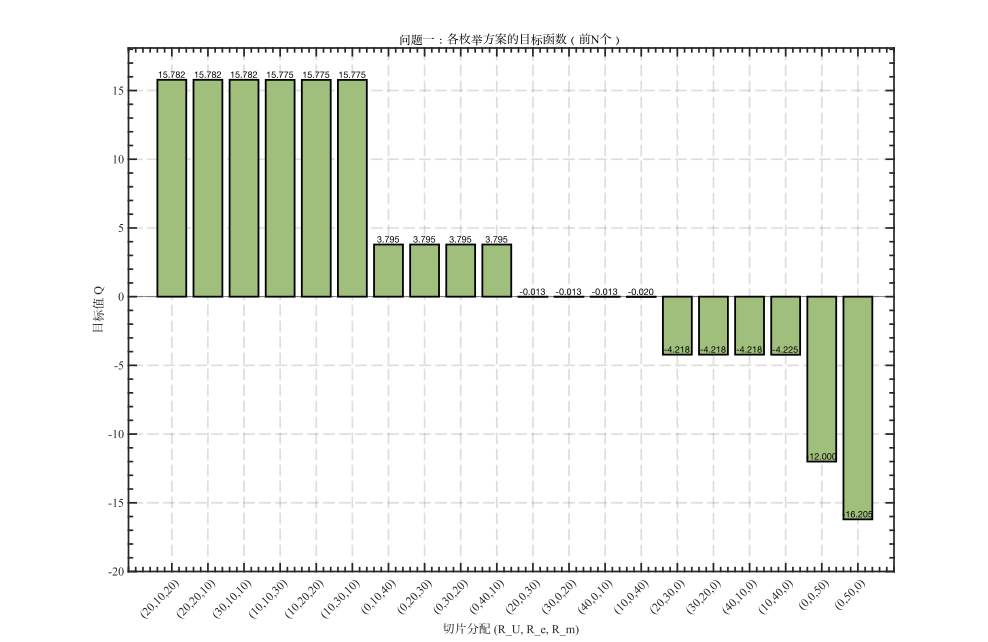
\includegraphics[width=0.8\textwidth]{figures/q1求解结果.pdf}
    \caption{第一问所有可行解枚举结果}
    \label{fig:q1_result}
\end{figure}
通过执行上述算法,我们枚举了所有可行解,如图\ref{fig:q1_result}所示。

\textbf{最优资源分配方案}

在所有结果中,我们找到了3个并列的最优资源分配方案,它们均能使系统总服务质量达到最大值15.7823。这三个方案的具体RB分配如下表所示。

\begin{table}[H]
\centering
\caption{并列最优资源分配方案}
\label{tab:q1_best_solutions}
\begin{tabular}{cccccc}
\hline
\textbf{方案} & \textbf{URLLC RB数 ($n_U$)} & \textbf{eMBB RB数 ($n_e$)} & \textbf{mMTC RB数 ($n_m$)} & \textbf{总QoS} \\
\hline
1 & 20 & 10 & 20 & 15.7823 \\
2 & 20 & 20 & 10 & 15.7823 \\
3 & 30 & 10 & 10 & 15.7823 \\
\hline
\end{tabular}
\end{table}

在以上三种方案中,各切片获得的QoS合计分数均相同,分别为:URLLC QoS合计1.9870,eMBB QoS合计3.7953,mMTC QoS合计10.0000。

 这三个方案均实现了资源的高效利用。在实际部署中,可以根据网络运营商的偏好进行选择。例如,方案1(20, 10, 20)为mMTC分配了最多的资源,适合未来mMTC连接数可能增加的场景;方案2(20, 20, 10)则向eMBB倾斜,适合视频流量大的场景;方案3(30, 10, 10)则最优先保障URLLC业务。这些方案共同构成了问题的最优解集。


综上所述,我们提出的资源分配方案能够有效满足各类切片用户的服务需求,实现了系统整体服务质量的最优。
\section{问题二的模型的建立和求解}
\subsection{问题二的描述与分析}

问题二考虑动态环境下的多时间段资源分配场景。与问题一的静态单时刻分配不同,问题二面临用户移动性、信道时变性以及任务队列动态变化的复杂问题。在1000ms的观测窗口内,系统需要每100ms进行一次资源分配决策(共10次),既要处理新到达的任务,又要考虑积压在排队队列中的历史任务。这是一个多阶段动态优化问题,需要在时间维度上综合考虑任务到达、信道变化和排队延迟的耦合影响。

\subsection{预备工作}
为便于复现与对比,本问采用如下统一的数据、参数与约定:

\begin{itemize}
  \item 数据来源(附件2,动态数据):任务到达流 \texttt{q2\_用户任务流.csv}(单位:Mbit,1ms时间粒度)、大规模衰减 \texttt{q2\_大规模衰减.csv}(单位:dB)、小规模瑞利衰减 \texttt{q2\_小规模瑞丽衰减.csv}(幅度 $|h|$)、用户位置 \texttt{q2\_用户位置.csv}(坐标信息)。按列名一一对应同名用户,忽略非数值列(如 \texttt{Time})。
  \item 决策周期:每100ms进行一次资源分配决策,共10个决策时刻:$t \in \{0, 100, 200, \ldots, 900\}$ ms。
  \item 系统与物理层参数:单小区、无同频干扰;发射功率 $p_{\text{tx}}=30\,\text{dBm}$;单RB带宽 $b=360\,\text{kHz}$;噪声系数 $NF=7\,\text{dB}$。白噪声按问题一相同公式计算。
  \item 资源占用粒度(同表1):URLLC/eMBB/mMTC 用户并发占用RB数分别为 $v_U=10$、$v_e=5$、$v_m=2$。约束切片RB分配满足 $n_U\bmod 10=0$、$n_e\bmod 5=0$、$n_m\bmod 2=0$,且 $n_U+n_e+n_m=50$。
  \item SLA与QoS:各切片的SLA参数、QoS函数定义与问题一完全一致。
  \item 任务处理机制:每个决策周期内,先服务队列中的历史任务(按FIFO顺序),再处理新到达任务;任务传输可跨越多个决策周期;超过SLA时延的任务立即丢弃并计入惩罚。
\end{itemize}

\subsection{模型建立}

\subsubsection{时变信道与传输速率模型}

在动态环境中,用户$k$在时刻$t$的接收功率需要考虑时变信道特性:

\begin{equation}
p_{\text{rx},k}(t) = 10^{\frac{p_{\text{tx}} - \phi_k(t)}{10}} \cdot |h_k(t)|^2 \quad \text{(mW)}
\end{equation}

其中,$\phi_k(t)$和$h_k(t)$分别为时刻$t$用户$k$的大规模衰减和小规模瑞利衰落系数。

相应地,用户$k$在时刻$t$获得$i_k(t)$个资源块时的传输速率为:

\begin{equation}
r_k(t) = i_k(t) \cdot b \cdot \log_2\left(1 + \frac{p_{\text{rx},k}(t)}{10^{\frac{N_0(i_k(t))}{10}}}\right) \quad \text{(bps)}
\end{equation}

\subsubsection{任务队列动态演化模型}

定义用户$k$在时刻$t$的任务队列状态:

\begin{itemize}
  \item $A_{k,\tau}(t)$:用户$k$在时刻$\tau$到达且在时刻$t$仍在队列中的任务数据量(Mbit)
  \item $Q_k(t) = \sum_{\tau=0}^{t} A_{k,\tau}(t)$:用户$k$在时刻$t$的总排队任务量
  \item $W_k(t)$:用户$k$在时刻$t$已等待的排队时间
\end{itemize}

任务队列的动态演化遵循以下规律:

\textbf{(1) 任务到达:}
在每个1ms时刻$\tau$,根据数据文件读取新到达任务:
\begin{equation}
A_{k,\tau}(\tau) = \text{TaskFlow}_k(\tau)
\end{equation}

\textbf{(2) 任务服务:}
在决策时刻$t$,若用户$k$被分配$i_k(t)$个RB,则在接下来的100ms内可传输的数据量为:
\begin{equation}
S_k(t) = r_k(t) \times 0.1 \times 10^{-6} \quad \text{(Mbit)}
\end{equation}

\textbf{(3) 队列更新:}
任务按FIFO顺序服务,队列更新规则为:
\begin{equation}
Q_k(t+100) = \max\left(0, Q_k(t) + \sum_{\tau=t+1}^{t+100} \text{TaskFlow}_k(\tau) - S_k(t)\right)
\end{equation}

\subsubsection{时延计算模型}

对于用户$k$在时刻$\tau$到达的任务,其总时延包含排队时延和传输时延:

\textbf{(1) 排队时延:}
任务在时刻$\tau$到达,在时刻$t_{\text{start}}$开始服务,则排队时延为:
\begin{equation}
Q_{k,\tau} = t_{\text{start}} - \tau
\end{equation}

\textbf{(2) 传输时延:}
假设任务从时刻$t_{\text{start}}$开始传输,数据量为$D_{k,\tau}$,则传输时延为:
\begin{equation}
T_{k,\tau} = \frac{D_{k,\tau} \times 10^6}{r_k(t_{\text{start}})}
\end{equation}

\textbf{(3) 总时延:}
\begin{equation}
L_{k,\tau}^s = Q_{k,\tau} + T_{k,\tau}, \quad s \in \{U, e, m\}
\end{equation}

\subsubsection{动态服务质量评估函数}

在多时间段场景下,各切片的QoS评估需要考虑所有完成任务的累积效果:

\textbf{(1) URLLC切片:}
对于在时间窗口$[0, 1000]$ms内完成的所有URLLC任务:
\begin{equation}
y_{k,\tau}^{U} = \begin{cases}
\alpha^{L_{k,\tau}^{U}} & \text{若 } L_{k,\tau}^{U} \leq L_{U}^{\text{SLA}} \\
-M_{U} & \text{若 } L_{k,\tau}^{U} > L_{U}^{\text{SLA}}
\end{cases}
\end{equation}

\textbf{(2) eMBB切片:}
对于在决策时刻$t$服务的eMBB用户$k$:
\begin{equation}
y_{k}^{e}(t) = \begin{cases}
1 & \text{若 } r_k(t) \geq r_{e}^{\text{SLA}} \text{ 且 } L_{k,\tau}^{e} \leq L_{e}^{\text{SLA}} \\
\frac{r_k(t)}{r_{e}^{\text{SLA}}} & \text{若 } r_k(t) < r_{e}^{\text{SLA}} \text{ 且 } L_{k,\tau}^{e} \leq L_{e}^{\text{SLA}} \\
-M_{e} & \text{若} L_{k,\tau}^{e} > L_{e}^{\text{SLA}}
\end{cases}
\end{equation}

\textbf{(3) mMTC切片:}
在每个决策时刻$t$,mMTC切片的QoS基于接入成功率:
\begin{equation}
y^{m}(t) = \frac{\sum_{k \in \mathcal{U}_{m}(t)} c_k'(t)}{\sum_{k \in \mathcal{U}_{m}(t)} c_k(t)}
\end{equation}
其中,$c_k(t)$表示用户$k$在时刻$t$是否有待服务任务,$c_k'(t)$表示是否成功接入服务。

\subsubsection{多时间段优化模型}

基于上述分析,建立如下多时间段动态优化模型:

\begin{equation}
\begin{aligned}
\max_{\{n_s(t)\}_{s,t}} \quad & Q_{i} = \sum_{t \in \mathcal{T}} \left[ \sum_{k \in \mathcal{U}_U} y_{k}^{U}(t) + \sum_{k \in \mathcal{U}_e} y_{k}^{e}(t) + y^{m}(t) \right]\\
\text{s.t.} \quad & \begin{cases}
 n_U(t) + n_e(t) + n_m(t) = 50 \\
 n_U(t) \bmod 10 = 0 \\
 n_e(t) \bmod 5 = 0  \\
 n_m(t) \bmod 2 = 0 \\
 Q_k(t+100) = \max(0, Q_k(t) + \Delta A_k(t) - S_k(t))\\
n_s(t) \geq 0 \\
\quad \forall t \in \mathcal{T},\quad \forall s \in \mathcal{S},\quad \forall k, t
 \end{cases}
 \end{aligned}
 \end{equation}
\begin{equation}
Q_{\text{total}} = \sum_{i=1}^{10} Q_{i}
\end{equation}
其中,$\mathcal{T} = \{0, 100, 200, \ldots, 900\}$为决策时刻集合,$i$为决策次数,$n_s(t)$为时刻$t$分配给切片$s$的RB数量,$Q_k(t)$为用户$k$在时刻$t$的排队任务量,$\Delta A_k(t)$为时间段$[t, t+100)$内用户$k$的新增任务量。

该模型的核心挑战在于:(1) 状态空间的指数级增长;(2) 任务到达的随机性与信道的时变性;(3) 排队时延与传输时延的耦合优化。需要设计高效的求解算法来处理这一复杂的多阶段随机优化问题。

\subsection{模型求解}

\textbf{Step1:} 

\textbf{Step2:} 

\textbf{Step3:} 

\subsection{求解结果}
\section{问题三的模型的建立和求解}
\subsection{问题三的描述与分析}

\subsection{预备工作}

\subsection{模型建立}

\subsubsection{集合、索引与参数}

为适配附件三的多微基站、同频复用且存在小区间干扰的场景,定义如下集合与索引:

\begin{itemize}
  \item 基站集合:$\mathcal{N}=\{1,2,3\}$(分别对应 BS1、BS2、BS3)。
  \item 切片集合:$\mathcal{S}=\{U,e,m\}$,分别对应 URLLC、eMBB、mMTC。
  \item 用户集合:$\mathcal{K}=\mathcal{K}_U\cup\mathcal{K}_e\cup\mathcal{K}_m$,其中 $\mathcal{K}_U=\{\mathrm{U1},\mathrm{U2}\}$,$\mathcal{K}_e=\{\mathrm{e1},\dots,\mathrm{e12}\}$,$\mathcal{K}_m=\{\mathrm{m1},\dots,\mathrm{m30}\}$。
  \item 决策时刻集合:$\mathcal{T}=\{0,100,\dots,900\}$(单位 ms),每个决策窗口长度为 $100$ ms;窗口内以 $1$ ms 步长进行链路与队列仿真,记窗口内细粒度时刻集合为 $\mathcal{F}(t)=\{t,t+1,\dots,t+99\}$。
\end{itemize}

关键系统参数(与问题一、二保持一致):

\begin{itemize}
  \item 每站可用 RB 总数 $R_{\text{tot}}=50$;单 RB 带宽 $b=360\,\mathrm{kHz}$;噪声系数 $NF=7\,\mathrm{dB}$;
  \item 切片占用粒度:$i_U=10,\ i_e=5,\ i_m=2$(每个并发用户占用的 RB 数);
  \item 发射功率决策范围(第三问):$p_{n,s}(t)\in[10,30]\,\mathrm{dBm}$,为“基站 $n$ 在窗口 $t$ 对切片 $s$ 的统一每 RB 功率”(切片内各 RB 功率一致)。
\end{itemize}

\subsubsection{信道与干扰模型}

附件三提供了每 $1$ ms 的大规模损耗 $\phi_{n,k}(\tau)$(dB)与小规模瑞利衰落 $h_{n,k}(\tau)$。设窗口 $t\in\mathcal{T}$ 内细粒度时刻为 $\tau\in\mathcal{F}(t)$,若用户 $k\in\mathcal{K}_s$ 在窗口 $t$ 由基站 $n$ 服务且被分配切片 $s$ 的 RB,则其接收功率(mW)为
\begin{equation}
 p_{\mathrm{rx},n\to k}(\tau)=10^{\frac{p_{n,s}(t)-\phi_{n,k}(\tau)}{10}}\cdot |h_{n,k}(\tau)|^2.
\end{equation}

噪声功率与占用 RB 数 $i$ 成正比,换算为线性功率(mW):
\begin{equation}
 N_0(i)=10^{\frac{-174+10\log_{10}(i\cdot b)+NF-30}{10}}.
\end{equation}

微基站同频复用引入同信道干扰。为保持“同一 RB 索引才互扰”的规则,我们令每站在窗口 $t$ 内将其 $50$ 个 RB 在频域上按切片连续划分且次序固定(例如 U-e-m),每个切片获得一段连续 RB 区间,跨站的相同 RB 索引构成同信道。于是用户 $k$ 的瞬时信干噪比为
\begin{equation}
 \gamma_k(\tau)=\frac{p_{\mathrm{rx},n\to k}(\tau)}{\sum\limits_{u\in\mathcal{N},\ u\neq n} I_{u\to k}(\tau)+N_0(i_s)},\quad s\in\mathcal{S},
\end{equation}
其中 $I_{u\to k}(\tau)$ 表示来自他站 $u$、在与 $k$ 所占 RB 索引重叠的切片 RB 上的干扰功率,按与上式相同的接收功率表达(由 $p_{u,s'}(t),\phi_{u,k}(\tau),h_{u,k}(\tau)$ 决定)。基于香农公式,窗口内瞬时速率为
\begin{equation}
 r_k(\tau)=i_s\cdot b\cdot \log_2\big(1+\gamma_k(\tau)\big)\quad(\mathrm{bps}).
\end{equation}

\subsubsection{任务到达与队列演化}

令 $D_{k}(\tau)\ge 0$ 表示 $1$ ms 时刻 $\tau$ 到达用户 $k$ 的任务数据量(Mbit,来自 taskflow 数据)。任务按 FIFO 服务。记 $Q_k(t)$ 为窗口起点 $t$ 的总排队量(Mbit)。若窗口 $t$ 内被服务的时隙集合为 $\mathcal{U}_k(t)\subseteq\mathcal{F}(t)$,则窗口内可传输的数据量为
\begin{equation}
 S_k(t)=\sum_{\tau\in\mathcal{U}_k(t)} r_k(\tau)\cdot 10^{-6}\cdot 10^{-3}\quad(\mathrm{Mbit}),
\end{equation}
其中 $10^{-3}$ 将 $\mathrm{bps}$ 与 $1$ ms 时长换算为 bit,再以 $10^{-6}$ 换算为 Mbit。窗口结束时队列更新为
\begin{equation}
 Q_k(t+100)=\max\Big\{0,\ Q_k(t)+\sum_{\tau\in\mathcal{F}(t)} D_k(\tau)-S_k(t)\Big\}.
\end{equation}

\subsubsection{RB 切片并发与调度规则}

令 $x_{n,s}(t)$ 为窗口 $t$ 时基站 $n$ 切片 $s$ 的 RB 数,满足 $\sum_{s\in\mathcal{S}}x_{n,s}(t)=R_{\text{tot}}$。切片 $s$ 的并发容量为
\begin{equation}
 C_{n,s}(t)=\big\lfloor x_{n,s}(t)/i_s\big\rfloor.
\end{equation}
窗口内采用“编号靠前优先”的串-并行调度:每个 $(n,s)$ 最多同时服务 $C_{n,s}(t)$ 个队头任务,任务完成即释放并补位。URLLC 在切片内可按紧迫度(距 SLA 的剩余时限)优先。

\subsubsection{QoS 评估函数}

与问题一、二一致,定义任务级 QoS:
\begin{equation}
 y^{U}_{k,\tau}=\begin{cases}
 \alpha^{L^{U}_{k,\tau}} & L^{U}_{k,\tau}\le L^{\text{SLA}}_{U}\\
 -M_U & \text{否则}
 \end{cases},\quad
 y^{e}_{k,\tau}=\begin{cases}
 1 & r_{k}(\tau_\text{srv})\ge r^{\text{SLA}}_{e}\ \&\ L^{e}_{k,\tau}\le L^{\text{SLA}}_{e}\\
 \dfrac{r_{k}(\tau_\text{srv})}{r^{\text{SLA}}_{e}} & r_{k}(\tau_\text{srv})< r^{\text{SLA}}_{e}\ \&\ L^{e}_{k,\tau}\le L^{\text{SLA}}_{e}\\
 -M_e & \text{否则}
 \end{cases}
\end{equation}
\begin{equation}
 y^{m}_{k,\tau}=\begin{cases}
 \dfrac{\sum\limits_{i\in\mathcal{K}_m}c'_i}{\sum\limits_{i\in\mathcal{K}_m}c_i} & L^{\,m}_{k,\tau}\le L^{\text{SLA}}_{m}\\
 -M_m & \text{否则}
 \end{cases}
\end{equation}
其中 $L^{s}_{k,\tau}=Q_{k,\tau}+T_{k,\tau}$ 为任务总时延,$\tau_\text{srv}$ 为其被服务时段代表点;$c_i,c'_i$ 分别表示 mMTC 的“有任务/成功接入”标记。SLA 与惩罚参数同问题一中表述:$\alpha=0.95$,$r^{\text{SLA}}_e=50\,\mathrm{Mbps}$,$L^{\text{SLA}}_{U}=5\,\mathrm{ms}$,$L^{\text{SLA}}_{e}=100\,\mathrm{ms}$,$L^{\text{SLA}}_{m}=500\,\mathrm{ms}$,$M_U=5, M_e=3, M_m=1$。

\subsubsection{决策变量与优化模型}

决策变量:
\begin{itemize}
  \item RB 切片分配:$x_{n,s}(t)\in\mathbb{Z}_{\ge 0}$;
  \item 发射功率:$p_{n,s}(t)\in[10,30]\,\mathrm{dBm}$;
  \item 接入关联:$a_{n,k}(t)\in\{0,1\}$,$\sum\limits_{n\in\mathcal{N}}a_{n,k}(t)\le 1$;若 $a_{n,k}(t)=1$ 则 $k$ 在窗口 $t$ 仅由站 $n$ 调度。
\end{itemize}

综合上述要素,第三问的动态联合优化模型可表述为(跨 10 个窗口聚合):
\begin{equation}
\begin{aligned}
\max_{\{x,p,a\}}\quad & Q_{\text{total}}=\sum_{t\in\mathcal{T}}\Bigg[\sum_{k\in\mathcal{K}_U}\sum_{\tau\in\mathcal{A}_k(t)} y^{U}_{k,\tau}+\sum_{k\in\mathcal{K}_e}\sum_{\tau\in\mathcal{A}_k(t)} y^{e}_{k,\tau}+\sum_{k\in\mathcal{K}_m}\sum_{\tau\in\mathcal{A}_k(t)} y^{m}_{k,\tau}\Bigg] \\
\text{s.t.}\quad & 
\left\{
\begin{aligned}
& \sum_{s\in\mathcal{S}} x_{n,s}(t)=50,\ \forall n\in\mathcal{N},\ t\in\mathcal{T}, \\
& x_{n,U}(t)\bmod 10=0,\ x_{n,e}(t)\bmod 5=0,\ x_{n,m}(t)\bmod 2=0, \\
& x_{n,s}(t)\in\mathbb{Z}_{\ge 0},\ \forall n,s,t, \\
& 10\,\mathrm{dBm}\le p_{n,s}(t)\le 30\,\mathrm{dBm},\ \forall n,s,t, \\
& \sum_{n\in\mathcal{N}} a_{n,k}(t)\le 1,\ a_{n,k}(t)\in\{0,1\},\ \forall k,t, \\
& r_k(\tau),\ \gamma_k(\tau)\ \text{由}\ (x,p,a)\ \text{与}\ (\phi,h)\ \text{及调度生成}, \\
& Q_k(t+100)=\max\Big\{0,\ Q_k(t)+\sum_{\tau\in\mathcal{F}(t)} D_k(\tau)-S_k(t)\Big\},\ \forall k,t.
\end{aligned}
\right.
\end{aligned}
\end{equation}
其中 $\mathcal{A}_k(t)\subseteq\mathcal{F}(t)$ 为窗口 $t$ 内属于用户 $k$ 且在 SLA 内完成的任务到达时刻集合;$r_k(\tau)$ 与 $S_k(t)$ 均受干扰耦合与调度影响,是 $(x,p,a)$ 的非线性函数。该模型体现了“多站同频干扰 + 切片化 RB 分配 + 切片级功率控制 + 任务队列”的耦合特性,属于带整数约束与非凸干扰项的时变 MINLP 问题。

\subsection{模型求解}

\textbf{Step1:} 

\textbf{Step2:} 

\textbf{Step3:} 

\subsection{求解结果}

%%%%%%%%%%%%%%%%%%%%%%%%%%%%%%%%%%%%%%%%%%%%%%%%%%%%%%%%%%%%%

\section{模型的分析与检验}

\subsection{灵敏度分析}

\subsection{误差分析}

%%%%%%%%%%%%%%%%%%%%%%%%%%%%%%%%%%%%%%%%%%%%%%%%%%%%%%%%%%%%%

\section{模型的评价}

\subsection{模型的优点}
\begin{itemize}[itemindent=2em]
\item 优点1
\item 优点2
\item 优点3
\end{itemize}

\subsection{模型的缺点}
\begin{itemize}[itemindent=2em]
\item 缺点1
\item 缺点2
\end{itemize}

%%%%%%%%%%%%%%%%%%%%%%%%%%%%%%%%%%%%%%%%%%%%%%%%%%%%%%%%%%%%%
%% 参考文献
\nocite{*}
\bibliographystyle{gbt7714-numerical}  % 引用格式
\bibliography{ref.bib}  % bib源

\newpage
%%%%%%%%%%%%%%%%%%%%%%%%%%%%%%%%%%%%%%%%%%%%%%%%%%%%%%%%%%%%%
%% 附录
\begin{appendices}
\section{文件列表}
\begin{table}[H]
\centering
\begin{tabularx}{\textwidth}{LL}
\toprule
文件名   & 功能描述 \\
\midrule
q1.m & 问题一程序代码 \\
q2.py & 问题二程序代码 \\
q3.c & 问题三程序代码 \\
q4.cpp & 问题四程序代码 \\
\bottomrule
\end{tabularx}
\label{tab:文件列表}
\end{table}

\section{代码}

\end{appendices}
\end{document}


%%%%%双图模板%%%%%%
\begin{figure}
\centering
\subcaptionbox{炉温曲线示意图\label{fig:双图a}}
{\includegraphics[width=.4\textwidth]{炉温曲线示意图.png}}
\subcaptionbox{问题1炉温曲线\label{fig:双图b}}
{\includegraphics[width=.4\textwidth]{问题1炉温曲线.png}}
\caption{双图}\label{fig:双图}
\end{figure} 
%%%%%双图模板%%%%%%